\chapter{Ciclo de vida y Participación de los usuarios en el proyecto}
\label{ch:ciclo de vida}


% El siguiente es el texto que aparece en el encabezamiento del proyecto fin de grado (si se quiere que sea distinto al nombre del capítulo))
\chaptermark{PFG}


\section{Ciclos de Baldugenda}
\label{secc:ciclos de Baldugenda}

En este apartado vamos a explicar el ciclo de vida y la participación de los usuarios. 
Los usuarios son un aspecto importante en el ciclo de vida del proyecto, en el desarrollo de proyectos dirigido a móviles, en los que el alumno no tiene experiencia previa y es un proyecto pensado por él, suele suceder que el proyecto se realice con fallos de diseño o con funcionalidades que los usuarios no ven necesarias y estos mismos usuarios echan en falta funcionalidades que sí que hubieran incluido si se les hubiera pedido opinión. 
Por este motivo, los usuarios tienen mucho peso durante las fases del ciclo de vida de éste proyecto.

El ciclo de vida que se decidió usar en el proyecto fue el siguiente, un modelo de ciclo de vida de desarrollo en espiral, se realizaron 3 ciclos principales en los cuales se iban añadiendo nuevos usuarios.
Para entender un poco más este concepto de ciclo de vida en espiral, primero hay que entender de qué trata. Si se compara con el desarrollo de un modelo en cascada, podemos ver que mientras en el modelo en cascada primero se buscan los requisitos, después se diseña la aplicación, se implementa y ya para finalizar se realizan las pruebas y el mantenimiento. 

En espiral primero se determinan objetivos que se quiere alcanzar en ese ciclo, tanto requisitos, como restricciones. Después se desarrollan la aplicación y se realizan las pruebas y una vez realizadas se planifica lo que se va a realizar para el siguiente ciclo y lo que se dejara fuera del proyecto. 

\begin{figure}[H] 
  \begin{center} 
    \scalebox{1}{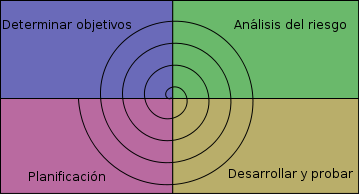
\includegraphics{figs/Espiral.png}} 
    \caption{Desarrollo en Espiral Wikipedia} 
    \label{fig:Espiral} 
  \end{center} 
\end{figure}

En cada ciclo se realizaban un alcance del proyecto y unas pruebas, el alcance y las pruebas realizadas en cada ciclo fueron las siguientes:

\subsection{Ciclo Uno}
\label{subsecc:ciclo Uno}

Para este ciclo los usuarios que estaban dentro del proyecto eran el tutor y el desarrollador de la aplicación. Las funcionalidades que se decidieron para este primer ciclo fueron los casos básicos referentes a la creación de asignaturas y exámenes, como son la creación de una asignatura con una lista de enlaces y la selección del tipo de evaluación que tiene la asignatura. En cuanto a los exámenes se pueden crear exámenes asociados a una asignatura con una fecha en concreto y la hora en la que se realizara el examen.
También se decidió incluir el API de Google Calendar al proyecto, y con el API se incluyeron más funcionalidades, la creación de un evento, dentro de un calendario de Google Calendar propiedad del usuario como recordatorio del examen. El usuario podría escoger si quiere notificaciones en ese evento o no, se agregó la  posibilidad de modificar los calendarios de Google propios del usuario dentro de la aplicación, y poder añadir o borrar calendarios existentes.
 
Dentro del ciclo aparte del alcance hubo una parte de pruebas donde tanto yo, el desarrollador hacia el rol de usuario de la aplicación y pasaba a ser un Balduser, y también el tutor sería un Balduser.


\subsection{Ciclo Dos}
\label{subsecc:ciclo Dos}

Después de realizar el ciclo uno se revisó las funcionalidades propuestas e implementadas durante el ciclo pasado. A la hora de realizar esta revisión se separaron las propuestas en 3 bloques, uno para las funcionalidades que se mantendrían o se implementarían para este ciclo (ciclo dos), en el segundo bloque estarían las funcionalidades que o por falta de tiempo o complejidad se dejarían para ciclos siguientes y en el bloque tres estarían las funcionalidades que quedarían fuera del proyecto porque se alejaban mucho de la idea inicial o por el coste que supondría hacerlas.
Las funcionalidades que se decidieron mantener de este primer ciclo fueron la mayor parte, al ser el primer ciclo, eran funcionalidades muy básicas como para poder desecharlas. Las implementaciones que se realizaron pero que no convencieron a los Baldusers de ese ciclo, se quitaron para el siguiente el siguiente ciclo y se decidió que si en el futuro hubiera tiempo se volverían a incluir. Una de las funcionalidades que sufrieron este cambio fue la de las notificaciones en los exámenes mediante Google Calendar. Durante el ciclo uno se implementó para ver su funcionamiento pero no convenció a los usuarios y se retiró para el comienzo del ciclo dos.

Para el alcance de este ciclo, los Baldusers agregados, probaron Baldugenda, y devolvieron el feedback sobre la aplicación que había resultado del ciclo uno. Dentro de este feedback se les pidió que dijeran funcionalidades nuevas que podrían añadirse en Baldugenda. Surgieron bastantes funcionalidades, como pasó en el ciclo uno se volvió a dividir esas funcionalidades en 3 bloques y durante la fase de determinar objetivos se escogió que funcionalidades se realizarían en este ciclo.
Para disponer de la información que devolvían los Baldusers de una manera rápida se decidio usar documentos de Google Drive y compartirlos a los Baldusers, ellos mismos irían rellenando lo que querían agregar a la aplicación y después en la fase de toma de decisiónes se escogería que se dejaba fuera.
En el bloque de los casos de uso que se realizarían durante este ciclo se agregó que los usuarios pudieran modificar una asignatura o un examen. Por otro lado también se decidió implementar el que el usuario pudiese borrar las asignaturas que no tuvieran exámenes asociados,  como aspectos nuevos que se incluirían en el ciclo dos fueron añadir nota en examen y en asignatura. Como también solucionar los errores encontrados por los Baldusers cuando estaban realizando el feedback. En el apartado de diseño los Baldusers se quejaron y ellos mismos propusieron un diseño que les parecía más atractivo.
Hubo casos de uso y aspectos que se tuvieron que dejar fuera como fue el caso de agregar aparte de exámenes, las tutorías, los trabajos grupales e individuales o los eventos.
Las funcionalidades que los Baldusers sugirieron y que parecieron interesantes pero se realizarían más adelante fueron la de agregar descripción en exámenes, y realizar unos ajustes en la aplicación para que cuando se crease un examen o una asignatura mostrara la asignatura o examen directamente sin tener que estar después buscándolo.

Durante la fase de análisis de riesgos se tuvo en cuenta que al ser una segunda versión de la aplicación, ya habría Baldusers que se la habían instalado y que en sus dispositivos estaba una versión de base de datos con un esquema distinto del que se lanzaría en la nueva versión, por este motivo lo primero que se llevaría a cabo seria el apartado de realizar una correcta transformación de la base de datos antigua a la nueva sin que los Baldusers perdieran la información almacenada hasta ese momento.
Para la parte de implementación se buscó la manera de que el usuario que probara la aplicación no se viera afectado con los cambios realizados, para conseguir ese objetivo el único aspecto de diseño que se modifico fue los iconos del menú principal.También a la hora de implementar los nuevos campos de nota en examen y en asignatura, se tenía que tener en cuenta tanto a los Baldusers que habían probado la aplicación como a los que la probarían en un futuro, por eso se tenía que seguir las dos situaciones que se podían dar cuando los usuarios probaran la nueva versión. Podía darse el caso que el usuario fuera nuevo o por el contrario ya la tuviera instalada y solo tuviera que actualizarla.

Para la fase de pruebas se les informo a los Baldusers que ya podían actualizar Baldugenda a la nueva versión con los cambios que habían solicitado. En ese momento los Baldusers tenían que realizar pruebas comprobar el diseño e informar de  cualquier fallo que se produjese en la aplicación. La fase de pruebas era una fase importante en este ciclo, ya que al haber agregado funcionalidades nuevas, tenían que funcionar correctamente si se quería empezar un ciclo nuevo sin problemas. Durante la fase de pruebas no se encontraron muchos fallos, los fallos que se encontraron se pudieron solucionar antes de comenzar el nuevo ciclo.

\subsection{Ciclo Tres}
\label{subsecc:ciclo Tres}

En este ciclo el funcionamiento vario con respecto a los anteriores, hay que recordar que durante el ciclo uno la cantidad de usuarios que podían usar la aplicación era un grupo reducido de 1 o 2 personas, en el ciclo dos el grupo de usuarios paso de ser 2 personas a ser 6 personas, y en el ciclo tres se volvió a aumentar el grupo de Baldusers y se probó con 15 personas.

Para empezar, en este ciclo se les permitió descargar la aplicación que se había desarrollado hasta el momento en el ciclo dos, y se les pidió el feedback, se cambió el método de adquirir la información de los Baldusers, ya que nos dimos cuenta que durante el ciclo dos el feedback producido por esos medios no fue suficientemente productivo. Por este motivo se les dio la posibilidad de ponerse en contacto conmigo tanto por teléfono, email o en persona para que me fueran informando de los cambios que veían necesarios para Baldugenda.
En algunos casos cuando el Balduser podía quedar conmigo se realizaron una serie de pruebas para saber cómo interactuaba con la aplicación, una de esas pruebas era la de tener que realizar una serie de acciones con Baldugenda y se le iban contando las pulsaciones que realizaba y el tiempo que le llevaba realizar cada tarea.
Los Baldusers respondieron mejor que la vez pasada aunque hubo más problemas a la hora de instalar la aplicación ya que el tipo de usuario que se escogió fue un tipo de usuario que no tenía conocimientos de informática, esto repercutió en el tiempo que necesitaban para instalarse la aplicación. Del feedback recibido por los Baldusers se incluyó en la implementación de este ciclo el apartado de poder realizar un backup de la información, para después poder recuperarla. También se agregó la descripción dentro de examen, esta funcionalidad la dijeron los usuarios del ciclo dos pero por tiempo no se pudo incluir. La mayoría de las funcionalidades que se modificaron fueron cambios en el funcionamiento en la interacción con la aplicación. Cambios del tipo pulsación de los botones o nuevos accesos a los casos de uso ya implementados. Se dejaron casos de uso fuera como fue el caso de modificar todo el diseño de la aplicación que se dejó para los siguientes ciclos.
 
En la fase de análisis de riesgos se tomó en cuenta que al querer implementar el backup con un servicio de Google, el API de Google Drive,  las dificultades que podían salir a la hora de trabajar con una tecnología que no se conocía de antes se solventarían atrasando el caso de uso del backup a un ciclo posterior, siempre y cuando las dificultades fueran tan importantes, en el caso de que no fuera así se buscaría una solución alternativa.

En la fase de implementación se desarrolló con éxito el apartado del backup con unos pequeños problemas al principio, los cuales por medio de documentación oficial se consiguió arreglar. Dentro de la fase de implementación se tuvo en cuenta que en ese momento podían existir 3 versiones de la aplicación, la versión del ciclo uno, la del ciclo dos y la versión actual del ciclo tres, así que había que tener cuidado con esa cuestión ya que la aplicación tenía que seguir funcionando daba igual de que versión se llegara. Cuando se acabó la implementación se subió a Google Play para compartir con los Baldusers la nueva versión, se la descargaron y realizaron unas pruebas para encontrar fallos. Todos los fallos que se fueron encontrando hasta la fecha se fueron resolviendo en una versión nueva cada semana.

El objetivo marcado para la finalizacion del ciclo tres, era una versión estable del producto, con las funcionalidades que se habían decidido incluir durante los tres ciclos. Apartir del tercer ciclo Baldugenda está recibiendo actualizaciones cuando los Baldusers encuentran fallos y se vuelve a subir una versión mejorada. 

% Mediante los siguientes comandos, podrás compilar el conjunto de ficheros desde este mismo documento


%%% Local Variables: 
%%% mode: latex
%%% TeX-master: "../Principal"
%%% End: 


















% line in order to check if utf-8 is properly configured: áéíóúñ